%!TEX root = ..\main.tex
%!TEX encoding = UTF-8 Unicode

%——————————————————————————————————————————————————————————-
%	CHAPTER 7
%——————————————————————————————————————————————————————————-
\newcommand\ue{\mathrm e}
\newcommand\sutw{$\mathcal{SU}(2)$}
\newcommand\suth{$\mathcal{SU}(3)$}
\newcommand\uo{$\mathcal{U}(1)$}
\newcommand\spint{自旋$\frac{1}{2}$}
\chapterimage{chapter_head_1.pdf} % Chapter heading image

\chapter[相互作用理论]{Interaction Theory\quad 相互作用理论}\label{chap7}

\section*{Summary\quad 总结}
在这一章中我们将导出不同的场之间的相互作用。这使得我们能够,例如,描述电子是如何和光子作用的%
\mpar{从另外一个视角看:电子(\spint 且有质量)场如何和光子(自旋为$1$)场作用。}。

内禀对称性,或者这里叫做规范%
\mpar{马上就会解释这个奇怪的名字}
对称性,能指引我们得到拉格朗日量的正确形式。我们将从局域%
\mpar{这意味着不仅仅是一个$\ue^{\ri\alpha}$,而是在每一个时空点上作用一个不同的因子,数学上写作$\ue^{\ri\alpha(x)}$。或者这样说:变换参数$\alpha=\alpha(x)$现在是$x$的函数,在不同的时空点上有不同的值。}%
$\mathcal{U}(1)$对称性出发来得到拉格朗日量
\[
{\mathscr L} = -m\bar\Psi\Psi+\ri\bar\Psi\gamma_\mu\partial^\mu\Psi + A_\mu\bar\Psi\gamma^\mu\Psi + \partial^\mu A^\nu\partial_\mu A_\nu - \partial^\mu A^\nu \partial_\nu A_\mu \text{,}
\]
即{\bf 量子电动力学(quantum electrodynamics)}的拉格朗日量。这个拉格朗日量描述了有电荷有质量的场和无质量自旋为$1$的场(光子场)之间的相互作用。在排除了形如$mA_\mu A^\mu$的“质量项”后(这和用$A_\mu$来描述的光子是无质量的实验事实相符),拉格朗日量只有这样才是局域$\mathcal{U}(1)$不变的%
\footnote{译注:应该为“只有这样才是且仅是”。}%
。利用 Noether 定理,我们能从\uo 对称性中导出一个新的守恒量,它常被解释为{\bf 电荷(electric charge)}。

接下来是$\mathcal{SU}(2)$对称性。引入一个二分量的{\bf 二重态(doublet)}
\[
\bar\Psi : = \begin{pmatrix}
\bar\psi_1 & \bar\psi_2
\end{pmatrix}\text{,}
\]
这样一个二重态场中包含了两个\spint 场,例如,电子和电子中微子场在$\mathcal{SU}(2)$的“旋转”下相互转换。

我们可以使用二重态记号写下局域$\mathcal{SU}(2)$不变的拉格朗日量%
\mpar{$W_j^{\mu\nu}$这玩意会通过三个$W_j^\mu$定义,就像从\uo 规范场$A^\mu$定义$F_{\mu\nu}$一样。}
\[
{\mathscr L} = \ri\bar\Psi\gamma_\mu\partial^\mu\Psi + \bar\Psi\gamma_\mu\sigma_j W_j^\mu\Psi - \frac{1}{2}(W_{\mu\nu})_i(W^{\mu\nu})_i \text{,}
\]
其中包含了三个自旋为$1$的场$W_j^\mu$。由于\sutw 群的生成元有三个基$J_i=\sigma_i/2$,所以我们需要三个场来保证拉格朗日量是局域\sutw 不变的。我们将看到局域\sutw 对称性仅当形如$m\bar\Psi\Psi$、$mW_\mu W^\mu$的质量项(其中质量$m$是任意给定{\bf 矩阵})不存在时才有可能实现,这是因为$\Psi$现在是二分量对象了。所以此时不仅自旋为$1$的场$W_j^\mu$得是无质量的了,\spint 场也一样。另外一种可能是两个\spint 等质量场,但是它被实验否决了:电子质量远大于电子中微子质量。除此之外,我们从实验知道三个自旋为$1$的场$W_j^\mu$不是无质量的。这常解释成\sutw 对称性被破缺了。

这是随后被引入的{\bf Higgs 机制(Higgs formalism)}的想法来源。这个机制能使我们得到一个包含质量项的\sutw 不变的拉格朗日量。它通过引入一个与零自旋场,即 Higgs 场,的相互作用来达成目标。相同的机制使我们能给\spint 场加上任意的质量项以与实验相符。最后的相互作用拉格朗日量描述了一种新的相互作用:{\bf 弱相互作用(weak interaction)},由三个%
\mpar{准确的讲:我们从${\mathcal U}(1)\otimes{\mathcal SU}(2)$对称破缺到\uo 。这个过程产生了三个有质量矢量 bosons:$W^+$、$W^-$、$Z$,和一个无质量矢量 bosons:$\gamma$光子。所以说为什么常讲电磁学(来自\uo 对称性)和弱相互作用理论(来自\sutw )是统一的。一开始的\uo 对称性和最后留下来的\uo 对称性不是一个东西。光子和$Z$Bosons可以看做是两个矢量Bosons的线性组合,常记做$B$和$W^3$,用以使拉格朗日量具有局域\uo ($B$波色子)和\sutw ($W^1$、$W^2$、$W^3$-bosons)不变性。}%
有质量自旋为$1$的场:$W^+$、$W^-$和$Z$,作为传播媒介。利用 Noether 定理,我们能从\sutw 对称性得到一个新的守恒量:{\bf 同位旋(isospin)},它相当于于电磁相互作用中的电荷,是弱相互作用中的荷。

最后,我们将考虑内禀\suth 对称,它将会将我们能描述一类新的相互作用,{\bf 强相互作用(strong interaction)},的拉格朗日量。为此我们将引入一个三重态
\[
Q = \begin{pmatrix}
q_1 \\
q_2 \\
q_3
\end{pmatrix}\text{,}
\]
在\suth 下变换,包含三个\spint 场。这三个\spint 场被解释为有不同{\bf 颜色(color)}的{\bf 夸克(quarks)},这是电磁作用中的电荷、或者弱作用中的同位旋在强相互作用中的对应物。一样,质量项是被禁止的,但这次和实验结论一致:8个相应的 bosons%
\mpar{数字8源于\suth 的生成元有8个基。}%
,称为胶子,是无质量的%
\mpar{作为补充,我们从实验知道\suth 的三重态中的场有相同的质量。这是个好消息,因为局域\suth 对称性禁止形如$m\bar QQ$这样带有任意质量矩阵$m$的项存在,但允许$\bar Q \begin{pmatrix}m&0\\ 0&m\end{pmatrix} Q$这样一项,这代表三重态里的项有相同的质量。由此局域\suth 不变性不会在拉格朗日量的质量项上造成新的障碍,\suth 对称也不没有被破缺。}%
。根据实验我们知道只有夸克(\spint )和胶子(自旋为$1$)携带颜色。最后,拉格朗日量的结果是
\[
{\mathscr L} = -\frac{1}{4}F_{\alpha\beta}^A F_A^{\alpha\beta} + \bar Q(\ri D_\mu\gamma^\mu - m)Q \text{,}
\]
咱仅仅引用一下\sout{装个逼},因为推导太繁琐了,并且和我们之前做过的完全类似。

给总结来总结一下:
\begin{table}[htbp]
\begin{tabular}{ccccccc}
 \uo & $\rightarrow$ & 1个规范场 & $\rightarrow$ & {\bf 无质量}光子 & $\rightarrow$ & 电荷 \\
 \sutw & $\rightarrow$ & 3个规范场 & $\rightarrow$ & {\bf 有质量}W- 和 Z-bosons (需要 Higgs ) & $\rightarrow$ & 同位旋 \\
 \suth & $\rightarrow$ & 8个规范场 & $\rightarrow$ & {\bf 无质量}胶子 & $\rightarrow$ & 色荷
\end{tabular}
\end{table}

\section[$\mathcal{U}(1)$相互作用]{$\mathcal{U}(1)$ Interaction\quad $\mathcal{U}(1)$相互作用}\label{sec7.1}
为了得到拉格朗日量中正确的相互作用项,我们得使用内禀对称性,或者称作{\bf 规范对称性(gauge symmetries)}。规范对称这个叫法有一些历史上的原因,和我们现在要讨论的东西之间关系不是太大。Weyl 曾尝试将电磁学%
\mpar{Frank Wilczek. Riemann-einstein structure from volume and gauge symmetry. Phys. Rev. Lett., 80:4851–4854, Jun 1998. doi: 10.1103/PhysRevLett.80.4851}%
“作为时空对称性的结果,特别是在局域尺度变换下的对称性”。将其称作规范对称性是有原因的,因为它意味着,例如,我们能任意改变用于定义长度标准的铂金尺(用来规范\footnote{译注:没有规矩,不成方圆。线长是某个线性空间中的某种范数,将改变线长的定义的变换,称作规范变换,应当是一个合理的称呼。关于 gauge 这个词的命名以及为何翻译成“规范”,可以参见 曹则贤 . Norm and Gauge[J]. 物理, 2013, 42(11): 815-819. }实验中测长的仪器),而不改变物理。这个尝试没有成功,但稍晚些时候,Weyl 找到了能正确导出电磁学的对称性,并仍用这个词来命名。

\subsection{\spint 自由场的内禀对称性}\label{sec7.1.1}
再来看一眼用来导出自由\spint 理论的拉格朗日量(\ref{eq:6.16}式)
\begin{equation}
{\mathscr L}_\text{Dirac} = -m\bar\Psi\Psi +\ri\bar\Psi\gamma_\mu\partial^\mu\Psi = \bar\Psi(\ri\gamma_\mu\partial^\mu-m)\Psi
\end{equation}
它是在 Lorentz 对称性的要求下导出的,但如果我们仔细观察它,能发现这个拉格朗日量中蕴含着另一个对称性。拉格朗日量在场$\Psi$的如下变换下不变
\begin{eqnarray}
\Psi &\rightarrow& \Psi' = \ue^{\ri a}\Psi \nonumber \\
\Rightarrow \bar\Psi &\rightarrow& \bar\Psi' = \Psi'^\dag \gamma_0 = (\ue^{\ri a}\Psi)^\dag \gamma_0 =\bar\Psi \ue^{-\ri a} \text{,}
\end{eqnarray}
其中负号来源于复共轭\mpar{别忘了$\bar\Psi=\Psi^\dag \gamma_0 $}%
,而$a$是一个任给实数。为了看清这一点,我们将变换后的场的拉格朗日量明确写出
\begin{eqnarray}
{\mathscr L}_\text{Dirac}' &=& -m\bar\Psi'\Psi' +\ri\bar\Psi'\gamma_\mu\partial^\mu\Psi' \nonumber\\
&=& -m(\bar\Psi \ue^{-\ri a})(\ue^{\ri a}\Psi)+\ri(\bar\Psi \ue^{-\ri a})\gamma_\mu\partial^\mu\Psi(\ue^{\ri a}\Psi) \nonumber\\
&=& -m\bar\Psi\Psi \underbrace{\ue^{-\ri a}\ue^{\ri a}}_{\mathclap{=1}} + \ri\bar\Psi\gamma_\mu\partial^\mu\Psi \underbrace{\ue^{-\ri a}\ue^{\ri a}}_{\mathclap{=1}} \nonumber\\
&=& -m\bar\Psi\Psi +\ri\bar\Psi\gamma_\mu\partial^\mu\Psi ={\mathscr L}_\text{Dirac}
\end{eqnarray}
其中我们利用了$\ue^{\ri a}$仅是一个复数这一点来将它自由前后挪动%
\mpar{技术上讲:一个复数和所有矩阵对易,例如$\gamma_\mu$。}%
。回忆我们在第\ref{chap3}章中曾讲过的,任何单位复数(能写作$\ue^{\ri a}$的形式)构成了一个\uo 群,由此可以将我们刚才发现的事实用数学语言表达出来:拉格朗日量是\uo 不变的。由于它丝毫不涉及时空的变换而只改变场自身,所以说这是一个内禀对称性。猛地一看,这玩意还挺萌的,但好像没什么用。不要走开,稍后的节目会告诉你它有多精彩!

现在咱再来钻深一点。我们刚展示了,给我们的场乘一个任意单位复数什么都不会改变。这个对称变换$\Psi \rightarrow \Psi' = \ue^{\ri a}\Psi$叫做{\bf 全局(global)}变换,因为我们在每一个点$x$给场$\Psi=\Psi(x)$乘上了一个相同的因子$\ue^{\ri a}$。

所以说,为什么一个时空点的相位因子会和另一个时空点的相关呢?一个点的选取不应该瞬间改变整个宇宙的情况。这是挺奇怪的,因为正如\ref{sec2.4}节中所述,狭义相对论告诉我们没有信息能比光传播得更快。而全局对称性选择会瞬间应用到在整个宇宙中的每一个点上%
\footnote{译注:引入局域规范的另一种讲法是,我们不能保证外星人里物理学家和我们选取同一套规范(这里的$a$是可以随意选取的,但是必须要选取一个才能得到完整的理论。$a$的选取被称为规范的选取),但是物理定律不应该有区别。}%
。

让我们来检查一下,如果给每一个时空点变换一个不同的因子$a=a(x)$,拉格朗日量是不是还是不变的。这叫做{\bf 局域(local)}变换。

我们作变换
\begin{eqnarray}
\Psi &\rightarrow& \Psi' = \ue^{\ri a(x)}\Psi \nonumber \\
\Rightarrow \bar\Psi &\rightarrow& \bar\Psi' = \Psi'^\dag \gamma_0 = (\ue^{\ri a(x)}\Psi)^\dag \gamma_0 =\bar\Psi \ue^{-\ri a(x)} \text{,}
\end{eqnarray}
现在$a=a(x)$依赖于坐标了,我们得到变换后的拉格朗日量%
\mpar{可能你会好奇包含全部可能导数项的拉格朗日量(由简洁性的要求被忽略)是不是局域\uo 不变的:${\mathscr L} = -m\bar\Psi\Psi +\ri\bar\Psi\gamma_\mu\partial^\mu\Psi+\ri(\partial^\mu\Psi)\gamma_\mu\Psi$。你可以检查一下,这个拉格朗日量自然是局域\uo 不变的,但注意第二项和第三项之和为零:$\ri\bar\Psi\gamma_\mu\partial^\mu\Psi+\ri(\partial^\mu\Psi)\gamma_\mu\Psi \underbrace{=}_{\mathclap{\text{分部积分}}} \ri(\partial^\mu\Psi)\gamma_\mu\Psi-\ri(\partial^\mu\Psi)\gamma_\mu\Psi = 0 $。包含了全部可能导数的正确拉格朗日量的两导数项间必须有一个相对负号:${\mathscr L_\text{Dirac}} = -m\bar\Psi\Psi +\ri\bar\Psi\gamma_\mu\partial^\mu\Psi-\ri(\partial^\mu\Psi)\gamma_\mu\Psi$,故它并{\bf 不}是局域\uo 不变的。
}
\begin{eqnarray}
{\mathscr L}_\text{Dirac}' &=& -m\bar\Psi'\Psi' +\ri\bar\Psi'\gamma_\mu\partial^\mu\Psi' \nonumber\\
&=& -m(\bar\Psi \underbrace{\ue^{-\ri a})(\ue^{\ri a}}_{\mathclap{=1}}\Psi)+\ri(\bar\Psi \ue^{-\ri a(x)})\gamma_\mu\partial^\mu\Psi(\ue^{\ri a(x)}\Psi) \nonumber\\
&=& -m\bar\Psi\Psi + \ri\bar\Psi\gamma_\mu\partial^\mu\Psi \underbrace{\ue^{-\ri a}\ue^{\ri a}}_{\mathclap{=1}} \underbrace{+}_{\mathclap{\text{莱布尼兹律}}} \ri(\ue^{-\ri a(x)}\bar\Psi)\gamma_\mu\Psi(\partial^\mu\ue^{\ri a(x)}) \nonumber\\
&=& -m\bar\Psi\Psi +\ri\bar\Psi\gamma_\mu\partial^\mu\Psi + \ri^2(\partial^\mu a(x))\bar\Psi\gamma_\mu\Psi \ne {\mathscr L}_\text{Dirac}
\label{eq:7.5}
\end{eqnarray}
由于莱布尼兹律导致了一个额外的项,所以说我们的拉格朗日量在局域\uo 对称变换下不是不变的。但按照上面所讨论的,拉格朗日量应该是局域不变的,在这里却不是。这里有一些事情可做,但我们得先研究另一种对称性。
\subsection{自旋为$1$自由场的内禀对称性}\label{sec7.1.2}
接下来,来看看自旋为一的粒子\mpar{对比\ref{eq:6.25}式,注意我们为了简明起见而丢掉的$\frac{1}{2}$因子}
\begin{equation}
{\mathscr L}_\text{Proca} = \partial^\mu A^\nu\partial_\mu A_\nu - \partial^\mu A^\nu \partial_\nu A_\mu + m^2A_\mu A^\mu \text{。}
\end{equation}
这儿也能找到一个全局内禀对称性。如果我们作变换
\begin{equation}
A_\mu \rightarrow A_\mu' = A_\mu+a_\mu
\end{equation}
其中$a_\mu$为任意常数,拉格朗日量变为
\begin{eqnarray}
{\mathscr L}_\text{Proca}' &=& \partial^\mu A'^\nu\partial_\mu A_\nu' - \partial^\mu A'^\nu \partial_\nu A_\mu' + m^2A_\mu' A'^\mu \nonumber\\
&=& \partial^\mu (A^\mu+a^\nu)\partial_\mu (A_\nu+a_\nu) - \partial^\mu (A^\nu+a^\nu) \partial_\nu ( A_\mu+a_\mu) + m^2( A_\mu+a_\mu) ( A^\mu+a^\mu) \nonumber\\
&=& \partial^\mu A^\nu\partial_\mu A_\nu - \partial^\mu A^\nu \partial_\nu A_\mu + m^2( A_\mu+a_\mu) ( A^\mu+a^\mu)
\end{eqnarray}
由此我们作出结论,对于{\bf 无质量}场($m=0$),这个变换是个{\bf 全局}对称的变换。

那{\bf 局域}对称性又会怎么样呢?作变换
\begin{equation}
A_\mu \rightarrow A_\mu' = A_\mu+a_\mu(x)
\end{equation}
{\bf 无质量}的拉格朗日量变成
\begin{eqnarray}
{\mathscr L}_\text{Maxwell}' &=& \partial^\mu A'\nu\partial_\mu A_\nu' - \partial^\mu A'\nu \partial_\nu A_\mu' \nonumber\\
&=& \partial^\mu (A^\mu+a^\nu(x))\partial_\mu (A_\nu+a_\nu(x)) - \partial^\mu (A^\nu+a^\nu(x)) \partial_\nu ( A_\mu+a_\mu(x))  \nonumber\\
&=& \partial^\mu A^\nu\partial_\mu A_\nu+\partial^\mu a^\nu(x)\partial_\mu A_\nu+\partial^\mu A^\nu\partial_\mu a_\nu(x) +\partial^\mu a^\nu(x)\partial_\mu a_\nu(x) \nonumber\\
& &\quad - \partial^\mu A^\nu \partial_\nu A_\mu - \partial^\mu A^\nu \partial_\nu a_\mu(x)-\partial^\mu a^\nu(x) \partial_\nu A_\mu - \partial^\mu a^\nu(x) \partial_\nu a_\mu(x)
\end{eqnarray}
即没有内禀对称性。

然而,如果我们这样作变换$A_\mu\rightarrow A_\mu'+\partial_\mu a(x)$,我们能弄出一个局域内禀对称性来。这意味着我们加的是一个任意函数的导数,而不是一个任意函数。这会导致\footnote{\textcolor{red}{译注:原文缺少一个$(x)$}}
\begin{eqnarray}
{\mathscr L}_\text{Maxwell}' &=& \partial^\mu A'\nu\partial_\mu A_\nu' - \partial^\mu A'\nu \partial_\nu A_\mu' \nonumber\\
&=& \partial^\mu (A^\mu+\partial^\nu a(x))\partial_\mu (A_\nu+\partial_\nu a(x)) - \partial^\mu (A^\nu+\partial^\nu a(x)) \partial_\nu ( A_\mu+\partial_\mu a(x))  \nonumber\\
&=& \partial^\mu A^\nu\partial_\mu A_\nu+\partial^\mu \partial^\nu a(x)\partial_\mu A_\nu+\partial^\mu A^\nu\partial_\mu \partial_\nu a(x) +\partial^\mu \partial^\nu a(x)\partial_\mu \partial_\nu a(x) \nonumber\\
& & - \partial^\mu A^\nu \partial_\nu A_\mu - \partial^\mu A^\nu \partial_\nu \partial_\mu a(x)-\partial^\mu \partial^\nu a(x) \partial_\nu A_\mu - \partial^\mu \partial^\nu a(x) \partial_\nu \partial_\mu a(x) \nonumber \\
&\underbrace{=}_{\mathclap{\partial_\nu\partial_\mu=\partial_\mu\partial_\nu\text{以及重命名哑指标}}}& \partial^\mu A^\nu\partial_\mu A_\nu - \partial^\mu A^\nu \partial_\nu A_\mu = {\mathscr L}_\text{Maxwell}\label{eq:7.11}
\end{eqnarray}
所以说这里的确有一个局域内禀对称变换。这看上去也像是一个技术细节。好的,我们找到了一些局域的、内禀的对称性,然后呢?
\subsection{把奇怪的东西堆一起}\label{sec7.1.3}
总结一下咱现在都干了啥
\begin{itemize}
\item 我们发现\spint 自由场的拉格朗日量有一个全局的内禀对称性$\Psi\rightarrow\Psi' = \ue^{\ri a}\Psi$。或者这样说:\spint 自由场的拉格朗日量在全局\uo 变换下不变。
\item 这个对称性不是局域的(尽管它应当是),因为在$a=a(x)$的情况下,我们在拉格朗日量中得到如下形式的额外项(\ref{eq:7.5}式)
\begin{equation}
-(\partial_\mu a(x))\bar\Psi\gamma^\mu\Psi \text{。}
\label{eq:7.12}
\end{equation}
换言之:拉格朗日量不是局域\uo 不变的。
\item 上一节中我们发现了无质量自旋为一的场的一个局域内禀对称性
\begin{equation}
A_\mu \rightarrow A_\mu' = A_\mu +\partial_\mu a(x) \text{,}
\label{eq:7.13}
\end{equation}
它仅当我们加上的是一个任意函数的导数$\partial_\mu a(x)$,而不是一个任意函数$a_\mu(x)$时,才是一个局域对称性。
\end{itemize}
这两坨奇怪的东西看上去真该加在一起:拉格朗日量中的一个额外项$A_\mu\bar\Psi\gamma^\mu\Psi$会变换作
\begin{equation}
A_\mu\bar\Psi\gamma^\mu\Psi \rightarrow (A_\mu+\partial_\mu a(x))\bar\Psi\gamma^\mu\Psi = A_\mu\bar\Psi\gamma^\mu\Psi + \partial_\mu a(x)\bar\Psi\gamma^\mu\Psi
\end{equation}
比较$\ref{eq:7.12}$式中的第二项\footnote{\textcolor{red}{译注:此处疑引用有误}}。拉格朗日量中这个将$\Psi$、$\bar\Psi$和$A_\mu$耦合在一起的新项,正好能干掉那个\sout{不自量力}阻挡\spint 自由场拥有局域\uo 不变性的家伙。换言之:{\bf 通过添加这个新项使得拉格朗日量局域\uo 不变。}

再来仔细研究一下这件事。首先习惯上都会在局域\uo 变换的指数上添一个常数因子$g$:$\ue^{\ri ga(x)}$。这样额外项变成
\begin{equation}
-(\partial_\mu a(x))\bar\Psi\gamma^\mu\Psi \rightarrow -g(\partial_\mu a(x))\bar\Psi\gamma^\mu\Psi \text{。}
\end{equation}
正如我们下面将看到的,这个额外的因子$g$代表一个任意的耦合常数%
\mpar{耦合常数总能告诉我们相互作用的强度是多少。这里讨论的是电磁相互作用,$g$代表着它的强度。}%
$g$。将这个新项
\[
g A_\mu\bar\Psi\gamma^\mu\Psi
\]
加到\spint 自由场的拉格朗日量上,其中$\gamma^\mu$用来保证这一项的 Lorentz 不变性,否则带有一个自由指标$\mu$的$A_\mu$和拉格朗日量密度这个标量无法匹配,另外也插入了{\bf 耦合常数(coupling constant)}%
\mpar{我们能看到这里$g$决定了$\Psi$、$\bar\Psi$和$A_\mu$耦合在一起的强度。}%
$g$。这样拉格朗日量
\[
{\mathscr L}_\text{Dirac+额外项} = -m\bar\Psi\Psi +\ri\bar\Psi\gamma_\mu\partial^\mu\Psi + g A_\mu\bar\Psi\gamma^\mu\Psi \text{。}
\]
依据$\Psi$、$\bar\Psi$和$A_\mu$局域变换的规则来变换这个拉格朗日量,得到%
\mpar{$\Psi$、$\bar\Psi$和$A_\mu$的联合变换被称作\uo {\bf 规范变换}。}
\begin{eqnarray}
{\mathscr L}_\text{Dirac+额外项}' &=& -m\bar\Psi'\Psi' +\ri\bar\Psi'\gamma_\mu\partial^\mu\Psi' + g A_\mu'\bar\Psi'\gamma^\mu\Psi' \nonumber\\
&\underbrace{=}_{\mathclap{\text{见\ref{eq:7.5}式}}}&  -m\bar\Psi\Psi +\ri\bar\Psi\gamma_\mu\partial^\mu\Psi - g (\partial_\mu a(x))\bar\Psi\gamma^\mu\Psi + g A_\mu'\bar\Psi'\gamma^\mu\Psi' \nonumber \\
&=& -m\bar\Psi\Psi +\ri\bar\Psi\gamma_\mu\partial^\mu\Psi - g (\partial_\mu a(x))\bar\Psi\gamma^\mu\Psi + g (A_\mu+\partial_\mu a(x))(\ue^{-\ri ga(x)}\bar\Psi)\gamma^\mu(\ue^{\ri ga(x)}\Psi) \nonumber \\
&=& -m\bar\Psi\Psi +\ri\bar\Psi\gamma_\mu\partial^\mu\Psi - \cancel{g (\partial_\mu a(x))\bar\Psi\gamma^\mu\Psi} + g A_\mu\bar\Psi\gamma^\mu\Psi + \cancel{g (\partial_\mu a(x))\bar\Psi\gamma^\mu\Psi}\nonumber \\
&=& -m\bar\Psi\Psi +\ri\bar\Psi\gamma_\mu\partial^\mu\Psi + g A_\mu\bar\Psi\gamma^\mu\Psi = {\mathscr L}_\text{Dirac+额外项} \text{。}
\end{eqnarray}

由此,在加上一个额外项后,我们得到了,正如所期待的,一个局域\uo 不变的拉格朗日量。为了描述一个包含了包含有质量\spint 场和无质量自旋为一的场的系统,我们必须将无质量自旋为一的自由场的拉格朗日量也加到拉格朗日量中来。这样就得到了完整的拉格朗日量
\begin{equation}
{\mathscr L}_\text{Dirac+额外项+Maxwell} = -m\bar\Psi\Psi +\ri\bar\Psi\gamma_\mu\partial^\mu\Psi + g A_\mu\bar\Psi\gamma^\mu\Psi + \partial^\mu A^\nu\partial_\mu A_\nu - \partial^\mu A^\nu \partial_\nu A_\mu \text{。}
\end{equation}
为了方便起见,引入记号
\begin{equation}
D_\mu \equiv \ri \partial_\mu + gA_\mu\text{,}
\end{equation}
称作{\bf 协变导数(covariant derivative)}\footnote{译注:常见的记号似乎与其差了一个虚数单位}。这样拉格朗日量写作
\begin{eqnarray}
{\mathscr L}_\text{Dirac+额外项+Maxwell} &=& -m\bar\Psi\Psi +\bar\Psi\gamma_\mu(\ri\partial^\mu+ g A^\mu)\Psi  + \partial^\mu A^\nu\partial_\mu A_\nu - \partial^\mu A^\nu \partial_\nu A_\mu \nonumber\\
&=& -m\bar\Psi\Psi +\bar\Psi\gamma_\mu D^\mu\Psi  + \partial^\mu A^\nu\partial_\mu A_\nu - \partial^\mu A^\nu \partial_\nu A_\mu
\end{eqnarray}
{\bf 这即为电磁场的量子场论,常被称为量子电动力学,的正确拉格朗日量}。我们通过观察\spint 自由场和自旋为一的自由场的内禀对称性,简单的得到了它。

我们将要回答的下一个问题是:这个拉格朗日量会导致什么样的运动方程?
\subsection{非齐次麦克斯韦方程和最小耦合}\label{sec7.1.4}
谜底揭晓:这个拉格朗日量给出有电流情况下的非齐次 Maxwell 方程组。

推导是很直白的:将拉格朗日量\footnote{\textcolor{red}{译注:原文下式标记有误,已更正。}}
\[
{\mathscr L}_\text{Dirac+额外项+Maxwell} = -m\bar\Psi\Psi +\ri\bar\Psi\gamma_\mu\partial^\mu\Psi + g A^\mu\bar\Psi\gamma_\mu\Psi + \partial^\mu A^\nu\partial_\mu A_\nu - \partial^\mu A^\nu \partial_\nu A_\mu
\]
代入每一个场的拉格朗日方程中
\[
\begin{aligned}
\frac{\partial \mathscr{L}}{\partial \Psi} - \partial_\mu \left( \frac{\partial \mathscr{L}}{\partial (\partial_\mu \Psi)} \right) &= 0 \\
\frac{\partial \mathscr{L}}{\partial \bar\Psi} - \partial_\mu \left( \frac{\partial \mathscr{L}}{\partial (\partial_\mu \bar\Psi)} \right) &= 0 \\
\frac{\partial \mathscr{L}}{\partial A_\rho} - \partial_\sigma \left( \frac{\partial \mathscr{L}}{\partial (\partial_\sigma A_\rho)} \right) &= 0 \text{。}
\end{aligned}
\]
得到
\begin{eqnarray}
\bar\Psi(\ri\gamma_\mu\partial^\mu + m)+gA_\mu\bar\Psi\gamma^\mu &=& 0 \\
(\ri\gamma_\mu\partial^\mu - m)\Psi-gA_\mu\gamma^\mu\Psi &=& 0 \label{eq:7.21} \\
\partial_\sigma(\partial^\sigma A^\rho - \partial^\rho A^\sigma) + g\bar\Psi\gamma^\rho\Psi &=& 0 \label{eq:7.22}
\end{eqnarray}
头两个方程描述了\spint 粒子/场在外加电磁场下的行为。在许多书里这些方程是利用一个叫做{\bf 最小耦合(minimal coupling)}的办法得到的,即当外场存在时,导数$\partial_\mu$应当换成协变导数%
\footnote{\textcolor{red}{译注:此处虚单位$\ri$的位置似有不妥,同后文}}
\begin{equation}
\partial_\mu \rightarrow D_\mu = \ri \partial_\mu + A_\mu
\end{equation}
来导出正确的方程。“最小”这个词的意思是,这里只用了一个规范场$A_\mu$的四个分量\footnote{译注:否则,我们可以使用张量场$\bar\Psi\sigma_{\mu\nu}F^{\mu\nu}\Psi$}。

现在我们有了用来描述 Dirac 旋量在外加电磁场中的行为的方程(\ref{eq:7.21}式),所以说可以来兑现在\ref{sec3.7.10}节中许下的承诺了。在那儿我们宣称电荷共轭变换,带有一个暗示性的名字,改变其描述对象的电荷。换言之,如果$\Psi$描述带电荷$+e$的某些东西,而电荷共轭旋量$\Psi^C$描述带电荷$-e$的某些东西。电荷决定了\spint 粒子/场和外加自旋为一的场的耦合强度,我们将考虑$\Psi^C$的运动方程是什么。之后我们将谈谈第三个方程,\ref{eq:7.22}式。
\subsection{再一次电荷共轭变换}\label{sec7.1.5}
为了得到对应的方程,我们需要找到 Dirac 旋量的电荷共轭变换算符确切的形式。我们在\ref{sec3.7.10}节中得到了变换(\ref{equ3.236}式)
\begin{equation}
\Psi = \begin{pmatrix}
\chi_L \\ \tilde\xi_R
\end{pmatrix} \rightarrow \Psi^C = \begin{pmatrix}
\tilde\xi_L \\ \chi_R
\end{pmatrix}\text{。}
\end{equation}
这个变换可以简单地用一个$\gamma_\mu$矩阵来描述。利用\ref{eq:6.13}式中$\gamma_2$的定义,我们有
\begin{equation}
\Psi^C = \ri\gamma_2 \Psi^* = \ri \begin{pmatrix}
0 & \sigma_2 \\
-\sigma_2 & 0\\
\end{pmatrix}\begin{pmatrix}
\chi_L^* \\ \tilde\xi_R^*
\end{pmatrix}\text{,}\label{eq:7.25}
\end{equation}
利用$\ri\sigma_2=\epsilon$正好就是旋量度规,改写作
\begin{equation}
\begin{pmatrix}
0 & \epsilon \\
-\epsilon & 0\\
\end{pmatrix}\begin{pmatrix}
\chi_L^* \\ \tilde\xi_R^*
\end{pmatrix}= \begin{pmatrix}
\epsilon\tilde\xi_R^* \\\epsilon\chi_L^*
\end{pmatrix} \text{。}
\end{equation}
等价于
\begin{equation}
= \begin{pmatrix}
\tilde\xi_L \\ \chi_R
\end{pmatrix}\text{,}
\end{equation}
正如\ref{sec3.7.7}节,特别是\ref{equ3.194}式中展示的一样。故我们从\ref{eq:7.21}式开始:
\begin{equation}
(\ri\gamma_\mu\partial^\mu - m)\Psi-gA_\mu\gamma^\mu\Psi = \left(\gamma_\mu(\ri\partial^\mu-gA^\mu) - m\right)\Psi = 0 \text{,}
\end{equation}
并取其复共轭,作为得到$\Psi^C$的方程的第一步:
\begin{equation}
\rightarrow \left(\gamma_\mu^*(-\ri\partial^\mu-gA^\mu) - m\right)\Psi^* = 0 \text{。}
\end{equation}
然后左乘一个$\gamma_2$,并在$\Psi$前插入一个$1=\gamma_2^{-1}\gamma_2$:
\begin{eqnarray}
& \rightarrow & \gamma_2\left(\gamma_\mu^*(-\ri\partial^\mu-gA^\mu) - m\right)\underbrace{\gamma_2^{-1}\gamma_2}_{=1}\Psi^* = 0 \text{。}\\
& \rightarrow & (\underbrace{\gamma_2\gamma_\mu^*\gamma_2^{-1}}_{=-\gamma_\mu}(-\ri\partial^\mu-gA^\mu) - m\gamma_2\gamma_2^{-1})\gamma_2\Psi^* = 0 \text{。}\\
& \underbrace{\rightarrow}_{\mathclap{\text{方程乘上}\ri}} & \left(-\gamma_\mu(-\ri\partial^\mu-gA^\mu) - m\right)\underbrace{\ri\gamma_2\Psi^*}_{\mathclap{=\Psi^C\text{见\ref{eq:7.25}式}}} = 0 \text{。}\\
& \rightarrow & \left(-\gamma_\mu(-\ri\partial^\mu-gA^\mu) - m\right)\Psi^C = 0 \text{,}
\end{eqnarray}
这和$\Psi$的运动方程只在耦合常数上差了个负号$g\rightarrow -g$。这与其名字,电荷共轭,相符%
\mpar{注意$\Psi^C\ne \bar\Psi$。$\Psi^C=\ri\gamma_2\Psi$而$\bar\Psi=\Psi^\dag\gamma_0=(\Psi^*)^T\gamma_0$。电荷共轭变换让我们能用反粒子来解释一些东西,稍后便会详细讨论。}。

接下来,我们转向上一节中的第三个式子,\ref{eq:7.22}式,称为{\bf 有电流情况下的非齐次麦克斯韦方程(inhomogeneous Maxwell equation in the presence of an electric current)}。为了讲清楚这个名字,我们又需要 Noether 定理了。
\subsection{内禀${\mathcal U}(1)$对称性的 Noether 定理}\label{sec7.1.6}
在\ref{sec4.5.5}节中我们得知 Noether 定理将所有内禀对称性和一个守恒量联系了起来。和我们刚才发现的\uo 对称性相联系的守恒量是什么?Neother 定理告诉我们,有如下形式的变换
\[
\Psi \rightarrow \Psi' = \Psi+\delta\Psi
\]
能导出 Noether 流
\[
J^\mu = \frac{\partial \mathscr L}{\partial(\partial_\mu\Psi)}\delta\Psi
\]
其满足连续性方程
\begin{equation}
\partial_\mu J^\mu =0\text{。}
\end{equation}
一个全局%
\mpar{记住,\spint 自由场的拉格朗日量仅仅是全局\uo 不变的。而上一节最终得到的拉格朗日量是全局\uo 不变的。全局对称性是局域对称性在$a=$常数时的特殊情况。所以说,如果我们有一个局域\uo 不变的拉格朗日量,它自动是全局\uo 不变的。这里考虑的全局\uo 对称性将导出一个对自由场和相互作用场都守恒的量}%
\uo 变换是
\[
\Psi \rightarrow \Psi' = \ue^{\ri ga} = (1+\ri ga+\dots)\Psi
\]
如通常所做的那样,我们仅将指数函数展开到第一项,因为\uo 是一个 Lie 群,而任意变换都可以由无穷小的来生成。一个无穷小的变换写作
\[
\Psi \rightarrow \Psi' = \Psi+\ri ga\Psi
\]
故我们有$\delta\Psi = \ri ga\Psi$。就如\ref{sec4.5.5}节中所做的一样,导出 Noether 流
\begin{eqnarray}
J^\mu &=& \frac{\partial \mathscr L}{\partial(\partial_\mu\Psi)}\delta\Psi \nonumber\\
&=& \frac{\partial( -m\bar\Psi\Psi +\ri\bar\Psi\gamma_\mu\partial^\mu\Psi)}{\partial(\partial_\mu\Psi)}\ri ga\Psi \nonumber\\
&=& -\bar\Psi\gamma^\mu ga\Psi =-ga \bar\Psi\gamma^\mu\Psi\text{。}
\end{eqnarray}
由于连续性方程对于任意$a$都成立,故略去%
\mpar{保留常数$g$,它的值由实验决定,而不是任意选取的。}%
任意的常数因子$a$。故,我们定义
\begin{equation}
J^\mu = -g\bar\Psi\gamma^\mu\Psi\label{eq:7.36}
\end{equation}
这常被称作{\bf 四电流(electric four-current)}。零分量正是电荷密度,其空间积分对时间守恒\mpar{类似的推导参见\ref{eq:4.39}式。}
\begin{equation}
Q = \int\rd^3\bm{x}\underbrace{\rho}_{\text{电荷密度}} = \int\rd^3\bm{x}~J^0 = -g\int\rd^3\bm{x} \bar\Psi\gamma^0\Psi
\end{equation}
在量子框架下,$\Psi$和概率幅相关,有要求$\int\rd^3\bm{x}~\bar\Psi\gamma^0\Psi=1$,即总概率必须为$100\%=1$。所以说守恒量实际就是耦合强度$g$,在电磁作用意义下正比于电荷。所以,全局\uo 对称性导致了电荷守恒。

注意\ref{eq:7.22}式,我们可以借助\ref{eq:7.36}式将其改写成
\begin{eqnarray}
\partial_\sigma(\partial^\sigma A^\rho - \partial^\rho A^\sigma) + \underbrace{g\bar\Psi\gamma^\rho\Psi}_{=-J^\rho} &=& 0 \nonumber\\
\rightarrow \partial_\sigma(\partial^\sigma A^\rho - \partial^\rho A^\sigma) &=& J^\rho\text{。}
\end{eqnarray}
借助\ref{eq:6.22}式中定义的电磁张量,改写作
\begin{equation}
\partial_\sigma F^{\rho\sigma} = J^\rho \text{。}
\end{equation}

这即是在有电流情况下的非齐次 Maxwell 方程组。这些方程组%
\mpar{“组”,因为对于每一个分量都有一个方程}%
,和非齐次 Maxwell 方程组(可以由$F^{\rho\sigma}$的定义直接得到%
\mpar{在\ref{chap11}章中将会见到}%
)一起,是经典电动力学的基础。

接下来我们将快速的过一遍有质量自旋为一的场和零自旋场的相互作用。
\subsection{零自旋有质量场的相互作用}\label{sec7.1.7}
注意我们导出的零自旋场的拉格朗日量
\[
{\mathscr L}= \frac{1}{2}(\partial_\mu\Phi\partial^\mu\Phi-m^2\Phi^2)
\]
不是\uo 不变的,做变换$\Phi\rightarrow\Phi'=\ue^{\ri a}\Phi$看一下就知道了。

但是,复标量理论
\begin{equation}
{\mathscr L}= \frac{1}{2}(\partial_\mu\Phi^*\partial^\mu\Phi-m^2\Phi^*\Phi)
\label{eq:7.40}
\end{equation}
具有\uo 对称性,因为有$\Phi\rightarrow\Phi'=\ue^{\ri a}\Phi$及$\Phi^*\rightarrow(\Phi^*)'=\ue^{-\ri a}\Phi^*$。所以我们有机会像\ref{sec7.1}节中对\spint 理论所做的那样,导出一个相互作用理论。推导完全是类似的%
\mpar{正确的拉格朗日量可以仅通过做替换$\partial_\mu \rightarrow D_\mu = \ri \partial_\mu + A_\mu$来得到}%
,结果是
\begin{equation}
{\mathscr L}= \frac{1}{2}\left(\left((\partial_\mu-\ri qA)\Phi^*\right)\left((\partial^\mu+\ri qA^\mu)\Phi\right)-m^2\Phi^*\Phi\right)
\label{eq:7.41}
\end{equation}
代入拉格朗日方程
\[
\begin{aligned}
\frac{\partial \mathscr{L}}{\partial \Phi} - \partial_\mu \left( \frac{\partial \mathscr{L}}{\partial (\partial_\mu \Phi)} \right) &= 0 \\
\frac{\partial \mathscr{L}}{\partial \Phi^*} - \partial_\mu \left( \frac{\partial \mathscr{L}}{\partial (\partial_\mu \Phi^*)} \right) &= 0\text{,}
\end{aligned}
\]
最终得到相应的运动方程\footnote{\textcolor{red}{译注:下式符号有误,已更正}}
\begin{eqnarray}
(\partial_\mu+\ri qA_\mu)(\partial^\mu-\ri qA^\mu)\Phi^*-m^2\Phi^*&=&0 \\
(\partial_\mu-\ri qA_\mu)(\partial^\mu+\ri qA^\mu)\Phi-m^2\Phi&=&0 \text{,}
\end{eqnarray}
描述了每一个零自旋场和自旋为一的无质量场相耦合。
\subsection{自旋为$1$有质量场的相互作用}\label{sec7.1.8}
自旋为$1${\bf 有质量}场和自旋为$1${\bf 无质量}场的相互作用也可以简单的由对称性得到。自旋为$1$无质量场的拉格朗日量为
\[
{\mathscr L}_\text{Maxwell} = \frac{1}{4}F^{\mu\nu}F_{\mu\nu} \text{。}
\]
为了区分有质量场和无质量场,我们将有质量场命名为$B^\mu$,并定义
\[
G^{\mu\nu} := \partial^\mu B^\nu - \partial^\nu B^\mu
\]
自旋为$1$的有质量场的拉格朗日量写作(\ref{eq:6.19}式)
\[
G_\text{Proca} = \frac{1}{2}G^{\mu\nu}G_{\mu\nu}+m^2 B^\mu B_\mu
\]
Lorentz 对称性说拉格朗日量中的相互作用项一定具有形式
\[
{\mathscr L}_\text{Procal-相互作用}=CG_{\mu\nu}F^{\mu\nu}
\]
其中耦合常数$C$需要由实验来定。感兴趣的读者可以借助欧拉-拉格朗日方程自行推导相应的运动方程。
\section[$\mathcal{SU}(2)$相互作用]{$\mathcal{SU}(2)$ Interaction\quad $\mathcal{SU}(2)$相互作用}\label{sec7.2}
\uo 对称性的成功激励着我们提出这个问题:\uo 对称性是我们的拉格朗日量唯一的内禀对称性吗?

事实上,我们能够在两个无质量\spint 粒子上找到另一个内禀对称性。我们将\ref{sec6.3}节中得到的拉格朗日量作两份加在一起,就是两个无质量\spint 粒子的拉格朗日量了。最后的结果即\ref{eq:6.16}式:
\[
{\mathscr L}_\text{Dirac} = \bar\psi(\ri\gamma_\mu\partial^\mu-m)\psi\text{。}
\]
这里我们将质量项略去,即$m=0$,否则马上就能看到拉格朗日量将不是变换不变的。再之后将看到我们是怎么在不破坏对称性的情况下把质量项捡回来的。“作两份加在一起”指的是
\begin{equation}
{\mathscr L}_{\text{D}_1+\text{D}_2} = \ri\bar\psi_1\gamma_\mu\partial^\mu\psi_1+\ri\bar\psi_2\gamma_\mu\partial^\mu\psi_2
\end{equation}
通过新定义{\bf 二重态(doublet)}$\Psi$
\[
\begin{aligned}
\Psi &:= \begin{pmatrix}
\psi_1 \\ \psi_2
\end{pmatrix} \\
\rightarrow \bar\Psi &:= \begin{pmatrix}
\bar\psi_1 & \bar\psi_2
\end{pmatrix}
\end{aligned}
\]
我们能将前式改写成
\begin{equation}
{\mathscr L}_{\text{D}_1+\text{D}_2} = \ri\bar\Psi\gamma_\mu\partial^\mu\Psi\text{。}
\end{equation}

这个拉格朗日量在{\bf 全局}\sutw 变换
\begin{eqnarray}
\Psi \rightarrow\Psi' &=& \ue^{\ri a_i \frac{\sigma_i}{2}}\Psi \\
\Rightarrow \bar\Psi \rightarrow\bar\Psi' &=& \bar\Psi\ue^{-\ri a_i \frac{\sigma_i}{2}} \text{,}
\end{eqnarray}
下不变。其中重复指标$i$代表求和,$a_i$为任意实数而$\frac{\sigma_i}{2}$是\sutw 群的常用生成元,$\sigma_i$是泡利矩阵。

为了看明白不变性,我们将变换后的拉格朗日量写出%
\mpar{这里我们丢掉了质量项。形如$-m_1\bar\Psi\Psi$和$-m_2\bar\Psi\Psi$的项可以借助$\Psi$的二分量定义和质量矩阵
\[
m:= \begin{pmatrix}
m_1 & 0 \\ 0 & m_2
\end{pmatrix}
\]
写作
\[
{\mathscr L}_{\text{D}_1+\text{D}_2} = -\bar\Psi m\Psi\text{。}
\]
不幸的是,这一项并不是\sutw 不变的,即
\[
{\mathscr L}'_{\text{D}_1+\text{D}_2} = -\bar\Psi' m\Psi'= \ri\bar\Psi\underbrace{\ue^{-\ri a_i \frac{\sigma_i}{2}}m\ue^{\ri a_i \frac{\sigma_i}{2}}}_{\ne m}\Psi\text{。}
\]
当质量相等$m_1=m_2$时,它自然是不变的,但是等会能看到我们可以在不违背对称性的情况下包含任意大小的质量。实验告诉我们二重态的两个场并没有产生相同质量的粒子,即$m_1\ne m_2$。稍后会有更加详细的讨论。}\footnote{\textcolor{red}{译注:原文边注公式缺一 prime ,已更正}}
\begin{equation}
\begin{aligned}
{\mathscr L}'_{\text{D}_1+\text{D}_2} &= \ri\bar\Psi'\gamma_\mu\partial^\mu\Psi' \\
&=\ri\bar\Psi\ue^{-\ri a_i \frac{\sigma_i}{2}}\gamma_\mu\partial^\mu\ue^{\ri a_i \frac{\sigma_i}{2}}\Psi \\
&=\ri\bar\Psi\gamma_\mu\partial^\mu\Psi = {\mathscr L}_{\text{D}_1+\text{D}_2}\text{,}\quad \checkmark
\end{aligned}
\end{equation}
最后一行源于我们的变换$\ue^{\ri a_i\frac{\sigma_i}{2}}$作用在我们的新定义的二分量对象$\Psi$上,而$\gamma_\mu$作用在二重态里面的对象上,即 Dirac 旋量%
\footnote{译注:用线性代数的话来讲,两个变换分别作用在两个子空间上,而这两个子空间的直积才是二重态所处的线性空间。}%
。我们可以用指标来将其写清楚\footnote{译注:指标真尼玛多。}
\[
\left[\left(\ue^{-\ri a_i\frac{\sigma_i}{2}}\right)_{ab}\delta_{\alpha\beta}\right]\left[\delta_{bc}\gamma_\mu^{\beta\delta}\right]\left[\left(\ue^{\ri a_i\frac{\sigma_i}{2}}\right)_{cd}\delta_{\delta\epsilon}\right]=\left[\delta_{ad}\gamma_\mu^{\alpha\beta}\right]
\]

这个对称性也该作为局域对称性。\sutw 变换将二重态的两个分量混合起来。稍后我们将会将这两个场称作电子和电子中微子场。对称性告诉我们,把哪个叫电子哪个叫电子中微子其实无所谓,因为用了\sutw 变换,想怎么换就怎么换。如果这仅仅是一个全局变换,那么当我们确定一个选择%
\mpar{这叫{\bf 规范选取(choosing a gauge)}。}%
,即哪个叫电子哪个叫电子中微子后,这个选择将瞬间适用到整个宇宙上去。故我们得研究局域变换。我们再一次发现它不是的,但正如局域\uo 对称性的情形一样,我们将尽最大努力让拉格朗日量具有局域\sutw 不变性。

问题依旧出在求导上,这会导致额外项:
\begin{equation}
\begin{aligned}
{\mathscr L}'_{\text{D}_1+\text{D}_2} &= \ri\bar\Psi'\gamma_\mu\partial^\mu\Psi' &\\
&=\ri\bar\Psi\ue^{-\ri a_i(x) \frac{\sigma_i}{2}}\gamma_\mu\partial^\mu\ue^{\ri a_i(x) \frac{\sigma_i}{2}}\Psi &\\
&=\ri\bar\Psi\gamma_\mu\partial^\mu\Psi-\bar\Psi\gamma_\mu\left(\partial^\mu a_i(x)\frac{\sigma_i}{2}\right)\Psi &\ne {\mathscr L}_{\text{D}_1+\text{D}_2}\text{。}
\end{aligned}
\end{equation}
有着\ref{sec7.1}节中处理\uo 的经验,我们很清楚接下来该做什么。我们将一步一步的导出一个局域\sutw 不变的拉格朗日量,这会花一些时间。为了避免读者陷入迷惑,在这里先列出接下来要进行的步骤:
\begin{itemize}
\item 最后的结论是,加上用以描述两个\spint 场$\begin{pmatrix} \psi_1\\ \psi_2 \end{pmatrix}$和三个有质量自旋为$1$的场$W_i^\mu$相互作用的额外项$\ri\bar\Psi\gamma_\mu W^\mu_i\sigma_i\Psi$后,拉格朗日量成为局域\sutw 不变的。
\item 注意,不变性仅当按照下式变换
\[
(W_\mu)_i\rightarrow (W'_\mu)_i=(W_\mu)_i+\partial_\mu a_i(x)+\epsilon_{ijk}a_j(x)(W_\mu)_k
\]
而不是
\[
(W_\mu)_i\rightarrow (W'_\mu)_i=(W_\mu)_i+\partial_\mu a_i(x)\text{,}
\]
即不同于\uo 对称性时的情况。
\item 仅当自由场拉格朗日量为如下形式\footnote{\textcolor{red}{译注:原文字体错误,已更正。}}
\[
{\mathscr L}=\frac{1}{4}(W_{\mu\nu})_i(W^{\mu\nu})^i
\]
其中
\[
(W_{\mu\nu})_i=\partial_\mu(W_\nu)_i-\partial_\nu(W_\mu)_i+\epsilon_{ijk}(W_\mu)_j(W_\nu)_k
\]
而不是
\[
(W_{\mu\nu})_i=\partial_\mu(W_\nu)_i-\partial_\nu(W_\mu)_i\text{。}
\]
时,对称性才存在。换言之,为了得到一个局域\sutw 不变的拉格朗日量,我们必须重新定义三个$W^\mu_i$场的拉格朗日量,使得其在变换
\[
(W_\mu)_i\rightarrow (W'_\mu)_i=(W_\mu)_i+\partial_\mu a_i(x)+\epsilon_{ijk}a_j(x)(W_\mu)_k
\]
下不变。
\end{itemize}

现在我们来具体执行这些步骤。从\ref{eq:7.11}式中我们得知自旋为$1$的场有内禀对称性
\[
A_\mu\rightarrow A'(x)+\partial_\mu a(x)
\]
而这里我们将会使用三个自旋为$1$的场$W_1^\mu,W_2^\mu$和$W_3^\mu$,这是因为\sutw 有三个生成元$\frac{\sigma_i}{2}$,由指数上的求和$a_i(x)\frac{\sigma_i}{2}$产生的每一个额外项都需要一个场。这导致了局域内禀对称性
\[
(W_\mu)_i\rightarrow (W'_\mu)_i=(W'_\mu)_i+\partial_\mu a_i(x)
\]
故我们尝试在拉格朗日量里添加项
\[
\bar\Psi\gamma_\mu\frac{\sigma_j}{2}W^\mu_j\Psi\text{。}
\]
不幸的是,这样并不能得到局域\sutw 不变的拉格朗日量%
\footnote{\textcolor{red}{译注:原文下式上下标混乱,以及最后两行漏$1/2$因子,以及倒数第二个等号应该为不等号,已更正。}}
\begin{equation}
\begin{aligned}
{\mathscr L}'_{\text{D}_1+\text{D}_2+\text{额外项}} &= \ri\bar\Psi'\gamma_\mu\partial^\mu\Psi'+\bar\Psi'\gamma_\mu\frac{\sigma_j}{2} {W'}_j^\mu \Psi' \\
&= \ri\bar\Psi\ue^{-\ri a_i(x)\frac{\sigma_i}{2}}\gamma_\mu\partial^\mu\ue^{\ri a_i(x)\frac{\sigma_i}{2}}\Psi \\
& \quad +\ri\bar\Psi\ue^{-\ri a_i(x)\frac{\sigma_i}{2}}\gamma_\mu\frac{\sigma_j}{2}\left(W_j^\mu+\partial^\mu a_j(x)\right)\ue^{\ri a_i(x)\frac{\sigma_i}{2}}\Psi \\
&= \ri\bar\Psi\gamma_\mu\partial^\mu\Psi - \bar\Psi\gamma_\mu\left(\partial^\mu a_i(x)\frac{\sigma_i}{2}\right)\Psi \\
& \quad + \bar\Psi\underbrace{\ue^{-\ri a_i(x)\frac{\sigma_i}{2}}\gamma_\mu\frac{\sigma_j}{2}W_j^\mu\ue^{\ri a_i(x)\frac{\sigma_i}{2}}}_{\mathclap{\ne \gamma_\mu\frac{\sigma_j}{2}W_j^\mu\text{因为}[\frac{\sigma_i}{2},\frac{\sigma_j}{2}]=\epsilon_{ijk}\frac{\sigma_k}{2}\ne 0 }} \Psi \\
& \quad +\ri\bar\Psi\ue^{-\ri a_i(x)\frac{\sigma_i}{2}}\gamma_\mu\frac{\sigma_j}{2}\left(\partial^\mu a_j(x)\right)\ue^{\ri a_i(x)\frac{\sigma_i}{2}}\Psi \\
&\ne \ri\bar\Psi\gamma_\mu\partial^\mu\Psi -\cancel{\bar\Psi\gamma_\mu\left(\partial^\mu a_i(x)\frac{\sigma_i}{2}\right)\Psi} + \bar\Psi\gamma_\mu\frac{\sigma_i}{2}W^\mu_i\Psi \\
& \quad + \cancel{\bar\Psi\gamma_\mu\left(\partial^\mu a_i(x)\frac{\sigma_i}{2}\right)\Psi} \\
&= \ri\bar\Psi\gamma_\mu\partial^\mu\Psi + \bar\Psi\gamma_\mu\frac{\sigma_i}{2}W^\mu_i\Psi = {\mathscr L}_{\text{D}_1+\text{D}_2+\text{额外项}} \quad \checkmark \label{eq:7.50}
\end{aligned}
\end{equation}
容易发现问题出在\sutw 的生成元不对易上%
\mpar{数学上将有非对易元素的群称为非阿贝尔的。作为对比,\uo 是阿贝尔的,此时一切都相对简单。}%
。我们来仔细研究一下这个困难。正如通常处理 Lie 群的那样,将目光集中在无穷小变换上,略去高阶项:
\begin{equation}
\begin{aligned}
\ue^{-\ri a_i(x)\frac{\sigma_i}{2}}\frac{\sigma_j}{2}\ue^{\ri a_i(x)\frac{\sigma_i}{2}} & = \left(1-\ri a_i(x)\frac{\sigma_i}{2}\right)\frac{\sigma_j}{2}\left(1+\ri a_i\frac{\sigma_i}{2}\right)\\
& = \frac{\sigma_j}{2}-a_i(x)\frac{\sigma_i}{2}\frac{\sigma_j}{2}+a_i(x)\frac{\sigma_j}{2}\frac{\sigma_i}{2}+{\mathcal O}(a^2)\\
& = \frac{\sigma_j}{2}+a_i(x)\left[\frac{\sigma_j}{2},\frac{\sigma_i}{2}\right]+{\mathcal O}(a^2)\\
& = \frac{\sigma_j}{2}-a_i(x)\epsilon_{ijk}\frac{\sigma_k}{2}+{\mathcal O}(a^2)\ne\frac{\sigma_j}{2} \label{eq:7.51}
\end{aligned}
\end{equation}
作为无穷小变换,${\mathcal O}(n^2)$和更高阶的项都可以略去,拉格朗日量为
\begin{equation}
\begin{aligned}
{\mathscr L}'_{\text{D}_1+\text{D}_2+\text{额外项}} &= \ri\bar\Psi'\gamma_\mu\partial^\mu\Psi'+\bar\Psi'\gamma_\mu\frac{\sigma_j}{2} {W'}_j^\mu \Psi' \\
&\underbrace{=}_{\mathclap{\text{\ref{eq:7.50}式}}} \ri\bar\Psi\gamma_\mu\partial^\mu\Psi - \bar\Psi\gamma_\mu\left(\partial^\mu a_i(x)\frac{\sigma_i}{2}\right)\Psi + \bar\Psi\ue^{-\ri a_i(x)\frac{\sigma_i}{2}}\gamma_\mu\frac{\sigma_j}{2}W_j^\mu\ue^{\ri a_i(x)\frac{\sigma_i}{2}} \Psi \\
&\quad  +\ri\bar\Psi\ue^{-\ri a_i(x)\frac{\sigma_i}{2}}\gamma_\mu\frac{\sigma_j}{2}\left(\partial^\mu a_j(x)\right)\ue^{\ri a_i(x)\frac{\sigma_i}{2}}\Psi \\
&\underbrace{\approx}_{\mathclap{\text{\ref{eq:7.51}式}}}\ri\bar\Psi\gamma_\mu\partial^\mu\Psi - \bar\Psi\gamma_\mu\left(\partial^\mu a_i(x)\frac{\sigma_i}{2}\right)\Psi + \bar\Psi\gamma_\mu \left(\frac{\sigma_j}{2}-a_i(x)\epsilon_{ijk}\frac{\sigma_k}{2}\right) W_j^\mu \Psi \\
&\quad  +\ri\bar\Psi\gamma_\mu\left(\frac{\sigma_j}{2}-a_i(x)\epsilon_{ijk}\frac{\sigma_k}{2}\right)\left(\partial^\mu a_j(x)\right)\Psi \\
&=\ri\bar\Psi\gamma_\mu\partial^\mu\Psi - \cancel{\bar\Psi\gamma_\mu\left(\partial^\mu a_i(x)\frac{\sigma_i}{2}\right)\Psi} + \bar\Psi\gamma_\mu \frac{\sigma_j}{2} W_j^\mu \Psi - \bar\Psi\gamma_\mu a_i(x)\epsilon_{ijk}\frac{\sigma_k}{2} W_j^\mu \Psi \\
&\quad + \cancel{\bar\Psi\gamma_\mu\left(\partial^\mu a_i(x)\frac{\sigma_i}{2}\right)\Psi} - \underbrace{\ri\bar\Psi\gamma_\mu a_i(x)\epsilon_{ijk}\frac{\sigma_k}{2}\left(\partial^\mu a_j(x)\right)\Psi}_{{\mathcal O}(a^2)} \\
&=\ri\bar\Psi\gamma_\mu\partial^\mu\Psi + \bar\Psi\gamma_\mu \frac{\sigma_j}{2} W_j^\mu \Psi - \bar\Psi\gamma_\mu a_i(x)\epsilon_{ijk}\frac{\sigma_k}{2} W_j^\mu \Psi \label{eq:7.52}
\end{aligned}
\end{equation}
属于$(W_\mu)_i$的能保证\sutw 不变的内禀对称性只能是
\[
(W_\mu)_i\rightarrow (W'_\mu)_i=(W_\mu)_i+\partial_\mu a_i(x)+\epsilon_{ijk}a_j(x)(W_\mu)_k
\]
因为它能够在拉格朗日量中添加一项,恰好抵消掉那个破坏对称性的家伙%
\footnote{\textcolor{red}{译注:原文上下标混乱,且等号注释位置有误,已更正。}}
\begin{equation}
\begin{aligned}
{\mathscr L}'_{\text{D}_1+\text{D}_2+\text{额外项}} &= \ri\bar\Psi'\gamma_\mu\partial^\mu\Psi'+\bar\Psi'\gamma_\mu\frac{\sigma_j}{2} {W'}_j^\mu \Psi' \\
&=\ri\bar\Psi\ue^{-\ri a_i(x)\frac{\sigma_i}{2}}\gamma_\mu\partial^\mu\ue^{\ri a_i(x)\frac{\sigma_i}{2}}\Psi \\
& \quad +\ri\bar\Psi\ue^{-\ri a_i(x)\frac{\sigma_i}{2}}\gamma_\mu\frac{\sigma_j}{2}\left(W_j^\mu+\partial^\mu a_j(x)+\epsilon_{jlm}a_l(x)(W^\mu)_m\right)\ue^{\ri a_i(x)\frac{\sigma_i}{2}}\Psi \\
&\underbrace{=}_{\mathclap{\text{\ref{eq:7.52}式}}} \ri\bar\Psi\gamma_\mu\partial^\mu\Psi + \bar\Psi\gamma_\mu \frac{\sigma_j}{2} W_j^\mu \Psi - \cancel{\bar\Psi\gamma_\mu a_i(x)\epsilon_{ijk}\frac{\sigma_k}{2} W_j^\mu \Psi} + \cancel{\bar\Psi\gamma_\mu \frac{\sigma_j}{2} \epsilon_{ilm}a_l(x) W_m^\mu \Psi} \\
&= {\mathscr L}_{\text{D}_1+\text{D}_2+\text{额外项}} \quad \checkmark
\end{aligned}
\end{equation}
接下来得看看这个到底是不是三个自旋为$1$的自由粒子的拉格朗日量的内禀对称性。三个自旋为$1$的粒子的拉格朗日量是
\begin{equation}
\begin{aligned}
{\mathscr L}_{3\times\text{Maxwell}} &= \frac{1}{4}(W^{\mu\nu})_1(W_{\mu\nu})_1+\frac{1}{4}(W^{\mu\nu})_2(W_{\mu\nu})_2+\frac{1}{4}(W^{\mu\nu})_3(W_{\mu\nu})_3\\
&=\frac{1}{4}(W^{\mu\nu})_i(W_{\mu\nu})_i
\end{aligned}
\end{equation}
其中
\begin{equation*}
(W_{\mu\nu})_i=\partial_\mu(W_\nu)_i-\partial_\nu(W_\mu)_i\text{。}
\end{equation*}

我们希望拉格朗日量在变换
\begin{equation}
(W_\mu)_i\rightarrow (W'_\mu)_i=(W'_\mu)_i+\partial_\mu a_i(x)+\epsilon_{ijk}a_j(x)(W_\mu)_k\label{eq:7.55}
\end{equation}
下不变。变换后的拉格朗日量是
\begin{equation}
\begin{aligned}
{\mathscr L}'_{3\times\text{Maxwell}} &= \frac{1}{4}(W'^{\mu\nu})_i(W'_{\mu\nu})_i \\
&\underbrace{=}_{\mathclap{\text{见\ref{eq:6.25}式}}} \partial^\mu(W'^\nu)_i\partial_\mu(W'_\nu)_i-\partial^\mu(W'^\nu)_i\partial_\nu(W'_\mu)_i \\
&= \partial^\mu\left((W^\nu)_i+\partial^\nu a_i(x)+\epsilon_{ijk}a_j(x)(W^\nu)_k\right)\partial_\mu\left((W_\nu)_i+\partial_\nu a_i(x)+\epsilon_{ijk}a_j(x)(W_\nu)_k\right) \\
&\quad\quad -\partial^\mu\left((W^\nu)_i+\partial^\nu a_i(x)+\epsilon_{ijk}a_j(x)(W^\nu)_k\right)\partial_\nu\left((W_\mu)_i+\partial_\mu a_i(x)+\epsilon_{ijk}a_j(x)(W_\mu)_k\right) \\
&\underbrace{=}_{\mathclap{\text{略去${\mathcal O}(a^2)$项}}} \partial^\mu(W^\mu)_i\partial_\mu(W_\nu)_i +\cancel{(\partial^\mu(W^\nu)_i)\partial_\mu\partial_\nu a_i(x)}+(\partial^\mu(W^\nu)_i)\partial_\mu\epsilon_{ijk} a_j(x)(W_\nu)_k \\
&\quad\quad +\cancel{\partial_\mu\partial_\nu a_i(x)(\partial^\mu(W^\nu)_i)} + \partial^\mu\epsilon_{ijk}a_j(x)(W^\nu)_k\partial_\mu(W_\nu)_i \\
&\quad\quad - \partial^\mu(W^\nu)_i\partial_\nu(W_\mu)_i - \cancel{(\partial^\mu(W^\nu)_i)\partial_\mu\partial_\nu a_i(x)} - \partial^\mu\epsilon_{ijk}a_j(x)(W^\nu)_k\partial_\nu(W_\mu)_i \\
&\quad\quad -\cancel{\partial_\mu\partial_\nu a_i(x)(\partial^\nu(W^\mu)_i)} - \partial_\mu\epsilon_{ijk}a_j(x)(W^\mu)_k\partial_\nu(W_\mu)_i \\
&= \underbrace{\partial^\mu(W^\nu)_i\partial_\mu(W_\nu)_i-\partial^\mu(W^\nu)_i\partial_\nu(W_\mu)_i}_{\mathclap{{\mathscr L}_{3\times\text{Maxwell}}}} + (\partial^\mu(W^\nu)_i)\partial_\mu\epsilon_{ijk} a_j(x)(W_\nu)_k \\
&\quad\quad +\partial^\mu\epsilon_{ijk}a_j(x)(W^\nu)_k\partial_\mu(W_\nu)_i - \partial^\mu\epsilon_{ijk}a_j(x)(W^\nu)_k\partial_\nu(W_\mu)_i - \partial^\mu\epsilon_{ijk}a_j(x)(W^\mu)_k\partial_\nu(W_\mu)_i \\
&\underbrace{=}_{\mathclap{\text{莱布尼兹律}}} {\mathscr L}_{3\times\text{自旋}1} - (\partial^\mu(W^\nu)_i)\epsilon_{ijk}(\partial_\mu a_j(x))(W_\nu)_k - (\partial^\mu\epsilon_{ijk}(W^\nu)_i)a_j(x)\partial_\mu(W_\nu)_k \\
&\quad\quad -\epsilon_{ijk}(\partial^\mu a_j(x))(W^\nu)_k\partial_\mu(W_\nu)_i - \epsilon_{ijk}a_j(x)(\partial^\mu (W^\nu)_k)\partial_\mu(W_\nu)_i \\
&\quad\quad + \partial^\mu(W_\mu)_i\epsilon_{ijk}(\partial_\nu a_j(x))(W^\nu)_k + \partial_\nu(W_\mu)_i\epsilon_{ijk}a_j(x)(\partial^\mu(W^\nu)_k) \\
&\quad\quad + \epsilon_{ijk}(\partial^\mu a_j(x))(W^\mu)_k\partial_\nu(W_\mu)_i + \epsilon_{ijk}a_j(x)(\partial^\mu(W^\mu)_k)\partial_\nu(W_\mu)_i
\end{aligned}
\end{equation}
显然没有内禀对称性。

尽管如此,我们可以通过在张量$W_{\mu\nu}$上加一个额外项
\[
-\epsilon_{ijk}(W_\mu)_j(W_\nu)_k
\]
来保证内禀对称性。即
\[
(W_{\mu\nu})_i=\partial_\mu(W_\nu)_i-\partial_\nu(W_\mu)_i-\epsilon_{ijk}(W_\mu)_j(W_\nu)_k\text{,}
\]
这样三个自旋$1$场便有了一个新的拉格朗日量%
\footnote{\textcolor{red}{译注:原文下式多一乘号,已更正}}
\begin{equation}
\begin{aligned}
{\mathscr L}_{3\times\text{Maxwell}} &=\frac{1}{4}(W_{\mu\nu})_i(W^{\mu\nu})_i \\
&= \left(\partial_\mu(W_\nu)_i-\partial_\nu(W_\mu)_i-\epsilon_{ijk}(W_\mu)_j(W_\nu)_k\right) \\
&\quad \times \left(\partial^\mu(W^\nu)_i-\partial^\nu(W^\mu)_i-\epsilon_{ijk}(W^\mu)_j(W^\nu)_k\right)
\end{aligned}
\end{equation}

读者可自行完成冗长的计算以验证拉格朗日量的不变性。综上,我们找到了局域\sutw 不变的拉格朗日量,写作
\begin{equation}
{\mathscr L}_{\text{D}_1+\text{D}_2+\text{相互作用}+3\times\text{Maxwell}} = \ri\bar\Psi\gamma_\mu\partial^\mu\Psi+\bar\Psi\gamma_\mu\frac{\sigma_j}{2} {W}_j^\mu \Psi - \frac{1}{4}(W_{\mu\nu})_i(W^{\mu\nu})_i
\end{equation}
\section[质量项、${\mathcal U}(1)$和$\mathcal{SU}(2)$的统一]{Mass Terms and Unification of ${\mathcal U}(1)$ and $\mathcal{SU}(2)$ \quad 质量项、${\mathcal U}(1)$和$\mathcal{SU}(2)$的统一}\label{sec7.3}
在上一章中,为了防止\sutw 对称性被破坏,我们不能往拉格朗日量中添加形如$m_1\bar\Psi\Psi$或$m_2(W_\mu)_i(W^\mu)_i$的质量项。而从实验中我们知道相应的粒子%
\mpar{例如,由$\Psi$描述的电子$e^-$和电子中微子$\nu_e$,以及由$(W_\mu)_i$描述的三个 bosons 。}%
却有质量,这常被解释为\sutw 对称性的破缺。这意味着对称性在高能标下存在,而在低能标下自发破缺。

之前我们得到了一个局域\uo 不变的拉格朗日量,在这里为方便起见我们将相应的自旋为$1$的场记做$B_\mu$:
\begin{equation}
{\mathscr L}_\text{局域\uo 不变} = -m\bar\psi\psi +\bar\psi\gamma_\mu(\ri\partial^\mu+ g B^\mu)\psi  -\frac{1}{4}B^{\mu\nu}B_{\mu\nu}
\end{equation}
其中
\[
B^{\mu\nu}:=\partial^\mu B^\nu-\partial^\nu B^\mu
\]
由于自旋为$1$的场$B^\mu$能保证拉格朗日量的\uo 不变性,所以其常被称作\uo {\bf 规范场}。

局域\sutw 不变的拉格朗日量是\mpar{之前为了简明起见略去的三个$W_i^\mu$场的耦合常数,现在记做$g'$。}
\[
{\mathscr L}_\text{局域\sutw 不变} = \bar\Psi\gamma_\mu(\ri\partial^\mu+g'\sigma_j W^\mu_j)\Psi - \frac{1}{4}(W_{\mu\nu})_i(W^{\mu\nu})_i
\]
其中
\[
(W_{\mu\nu})_i = \partial_\mu(W_\nu)_i - \partial_\nu(W_\mu)_i + \epsilon_{ijk}(W_\mu)_j(W_\nu)_k
\]
以及二重态
\[
\Psi := \begin{pmatrix}
\psi_1 \\ \psi_2
\end{pmatrix}
\]
类似的,由于这三个自旋为$1$的场$(W_\nu)_i$能保证拉格朗日量的局域\sutw 不变性,故其常被称为\sutw 规范场。

将它们加到一起我们能得到一个局域\uo {\bf 且}\sutw 不变的拉格朗日量
\begin{equation}
{\mathscr L}_\text{\sutw 且\uo} = \bar\Psi\gamma_\mu(\ri\partial^\mu+ g B^\mu+g'\sigma_j W^\mu_j)\Psi - \frac{1}{4}(W_{\mu\nu})_i(W^{\mu\nu})_i -\frac{1}{4}B^{\mu\nu}B_{\mu\nu}\text{。}
\end{equation}

现在,该怎么在不破坏\sutw 对称性的前提下加入质量项呢?至今我们还没用过的唯一一个东西是零自旋场,所以来看看这个。零自旋场具有全局\uo 不变性的拉格朗日量由\ref{eq:7.40}式给出
\begin{equation}
{\mathscr L}_\text{零自旋} = \frac{1}{2}\left(\partial_\mu\phi^\dag\partial^\mu\phi - m^2\phi^\dag\phi\right)\text{。}
\end{equation}
我们还能在不破坏任何对称约束的情况下在这个拉格朗日量中添加$\phi$的高阶项%
\mpar{记住,唯一真正禁止的是高阶导数项,否则无法得到合理的理论。$\phi$的高幂次项描述场$\phi$的自作用,在希望得到一个“自由”理论的时候被略去。}%
。故我们写出下式,其中常数改作了惯用的记号
\begin{equation}
{\mathscr L}_\text{零自旋+额外项} = \partial_\mu\phi^\dag\partial^\mu\phi + \rho^2\phi^\dag\phi - \lambda^2(\phi^\dag\phi)^2\text{。}
\end{equation}
从\ref{eq:7.41}已经得知如何在使拉格朗日量局域\uo 不变的前提下,在零自旋场和\uo 规范场$B_\mu$间添加耦合项:
\begin{equation}
\begin{aligned}
{\mathscr L}_\text{零自旋+额外项+自旋1耦合} &= (\partial_\mu-\ri\frac{1}{2}gB_\mu)\phi^\dag(\partial^\mu+\ri\frac{1}{2}gB^\mu)\phi \\
 &+ \rho^2\phi^\dag\phi - \lambda^2(\phi^\dag\phi)^2
\label{eq:7.63}
\end{aligned}
\end{equation}
其具有对称性%
\mpar{见\ref{eq:7.13}式,并记得整体乘在拉格朗日量上的一个常数不会影响物理。}
\begin{eqnarray}
B_\mu &\rightarrow B_\mu' &= B_\mu+\partial_\mu a(x) \\
\phi(x) &\rightarrow \phi'(x) &= \ue^{\ri a(x)}\phi(x) \text{。}
\end{eqnarray}

用我们在上一节中对\spint 场导出局域\sutw 不变拉格朗日量同样的办法,我们能对零自旋场的二重态%
\mpar{\(\Phi = \begin{pmatrix} \phi_1 \\ \phi_2 \end{pmatrix}\)}%
写出一个局域\sutw 不变的拉格朗日量
\begin{equation}
\begin{aligned}
{\mathscr L}_\text{\sutw 且\uo} &= (\partial_\mu-\ri g'\sigma_i(W_\mu)_i-\ri\frac{1}{2}gB_\mu)\Phi^\dag(\partial^\mu+\ri g'\sigma_i(W^\mu)_i+\ri\frac{1}{2}gB^\mu)\Phi \\
 &+ \underbrace{\rho^2\Phi^\dag\Phi - \lambda^2(\Phi^\dag\Phi)^2}_{\equiv -V(\Phi)}
\label{eq:7.66}
\end{aligned}
\end{equation}
其中\(\Phi := \begin{pmatrix} \phi_1 \\ \phi_2 \end{pmatrix}\),对称变换为(\ref{eq:7.55}式)
\begin{equation}
(W_\mu)_i\rightarrow (W'_\mu)_i=(W'_\mu)_i+\partial_\mu b_i(x)+\epsilon_{ijk}b_j(x)(W_\mu)_k
\end{equation}
和
\begin{equation}
\Phi \rightarrow \Phi' = \ue^{\ri b_i(x)\sigma_i}\Phi, \quad \bar\Phi \rightarrow \bar\Phi' = \bar\Phi\ue^{-\ri b_i(x)\sigma_i}
\end{equation}

我们从局域\sutw 不变的拉格朗日量出发,研究它是如何为场$(W_\mu)_i$和$(B_\mu)_i$给出质量项的。手动添加质量项是不可行的, 因为它会破坏对称性从而导致不可接受的理论%
\mpar{这个理由很复杂,具体讨论不会在本书中给出。技术上讲:我们需要一个局域\sutw 对称的拉格朗日量来得到一个可重整的理论。感兴趣的读者可以参阅本节末给出的参考书目。}。

我们在上面定义了
\begin{equation}
\begin{aligned}
V(\Phi) &= -\rho^2 \Phi^\dag\Phi + \lambda(\Phi^\dag\Phi)^2\\
 &= -\rho^2\phi_1^\dag\phi_1 + \lambda(\phi_1^\dag\phi_1)^2 -\rho^2\phi_2^\dag\phi_2 + \lambda(\phi_2^\dag\phi_2)^2 \\
 &= V(\phi_1) + V(\phi_2)
\label{eq:7.69}
\end{aligned}
\end{equation}
这常称作 Higgs 势。其参数$\rho$取不同值而$\lambda$取正的图绘制于图\ref{fig:7.1}
\marginpar{
	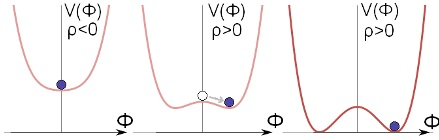
\includegraphics[width=0.4\textwidth]{./Figure/fig7_1.jpg}
	\figcaption{Higgs 势取不同参数$\rho$值的图像,$\rho$被认为是由于宇宙暴涨所造成的宇宙冷却而改变。Figure adapted from ``Spontaneous symmetry breaking'' by FT2 (Wikimedia Commons) released under a CC BY-SA 3.0 licence: \url{http://creativecommons.org/licenses/by-sa/3.0/deed.en}. URL:\url{http://commons.wikimedia.org/wiki/File:Spontaneous_symmetry_breaking_(explanatory_diagram).png}, Accessed: 8.12.2014}
	\label{fig:7.1}
}

这个想法是这样的:在相当高的温度下,例如宇宙早期,势能会像图左那样。极小值点,这里成为真空值,毫无疑问的在$\phi=0$处。参数$\lambda$和$\rho$随着温度的下降发生改变,势能的形状也是一样。当温度低于某个临界值时,如图右所示,$\phi=0$处不再是极小点。此时将会有许多点都能取到极小值。

事实上,这个势能有无穷多个极小值点。其可用通常的办法计算得到
\begin{eqnarray}
&V(\phi) = -\rho^2|\phi|^2 + \lambda |\phi|^4 \\
&\frac{\partial V(\phi)}{\partial \phi} = -2\rho^2|\phi|+4\lambda|\phi|^3 \\
\rightarrow &|\phi|(-2\rho^2+4\lambda|\phi|^2) \overset{\text{!}}{=} 0\\
\rightarrow &|\phi|^2  \overset{\text{!}}{=} \frac{\rho^2}{2\lambda} \\
\rightarrow &|\phi|  \overset{\text{!}}{=} \sqrt{\frac{\rho^2}{2\lambda}} \\
&\phi_{\min} = \sqrt{\frac{\rho^2}{2\lambda}} \ue^{\ri {\varphi}}\text{。}
\end{eqnarray}
这对于$\varphi$的任意取值都是极小值,所以我们有无穷多个极小点。全体极小点躺在了半径为$\sqrt{\frac{\rho^2}{2\lambda}}$的一个圆上。图\ref{fig:7.2}即为 Higgs 的三维图。就如同一粒弹珠从墨西哥草帽顶端自发而随机的滚落,一个新的真空值有无穷多种选择。
\marginpar{
	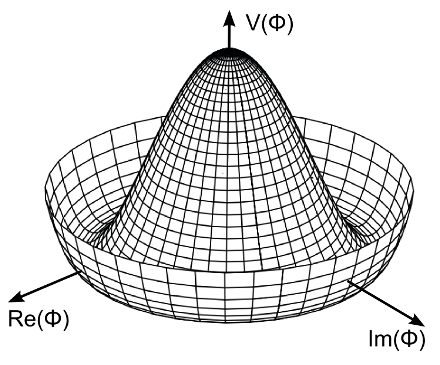
\includegraphics[width=0.4\textwidth]{Figure/fig7_2.png}
	\figcaption{Higgs 的三维图。 Figure adapted from ``Mexican hat potential polar'' by Rupert Millard (Wikimedia Commons) released under a public domain licence. URL:\url{http://commons.wikimedia.org/wiki/File:Mexican_hat_potential_polar.svg}, Accessed: 7.5.2014}
	\label{fig:7.2}
}

从\ref{eq:7.69}中我们可知对于二重态,两个分量都需要作出这种选择。则对于二重态其极小点为
\begin{equation}
\Phi_{\min} = \begin{pmatrix}
\phi_{1\min} \\ \phi_{2\min}
\end{pmatrix}
\end{equation}
一个经济的{\bf 选择}%
\mpar{复习:对称破缺意味着{\bf 一个}极小值有无穷多种选取方式}%
是
\begin{equation}
\Phi_{\min} = \begin{pmatrix}
0 \\ \sqrt{\frac{\rho^2}{2\lambda}}
\end{pmatrix} \equiv \begin{pmatrix}
0 \\ \frac{v}{\sqrt{2}}
\end{pmatrix} \text{,}
\end{equation}
其中因子$\frac{1}{2}$只是为了使计算简洁而引入,自然有$v\equiv\sqrt{\frac{\rho^2}{\lambda}}$。下一步中我们会将场$\Phi$在极小值附近展开以得到我们想要的物理。之后我们将会学到,由于得不到精确解,量子场论中的计算总是围绕着极小值点的一系列级数。为了得到有意义的结果,我们必须将场移动到新的极小点。故我们考虑
\begin{equation}
\Phi = \begin{pmatrix}
\phi_{1r}+\ri \phi_{1c} \\ \frac{v}{\sqrt{2}}\phi_{2r}+\ri \phi_{2c}
\end{pmatrix}\text{。}
\end{equation}

改写作\mpar{等会就能看到这个形式有多有用了。}
\begin{equation}
\Phi = \ue^{\ri \theta_i \frac{\sigma_i}{2}} \begin{pmatrix}
0 \\ \frac{v+h}{\sqrt{2}}
\end{pmatrix}\text{,}
\label{eq:7.79}
\end{equation}
这是由于考虑将指数函数展开成级数,代入泡利矩阵$\sigma_i$矩阵的具体形式,在一阶意义上
\begin{equation}
\begin{aligned}
\ue^{\ri \theta_i \frac{\sigma_i}{2}} \begin{pmatrix}
0 \\ \frac{v+h}{\sqrt{2}}
\end{pmatrix} &\approx (1+\ri \theta_i \frac{\sigma_i}{2}) \begin{pmatrix}
0 \\ \frac{v+h}{\sqrt{2}}
\end{pmatrix} \\
 &= (1+\ri \theta_1 \frac{\sigma_1}{2}+\ri \theta_2 \frac{\sigma_2}{2}+\ri \theta_3 \frac{\sigma_3}{2}) \begin{pmatrix}
0 \\ \frac{v+h}{\sqrt{2}}
\end{pmatrix} \\
 &= \begin{pmatrix}
 1 + \ri\frac{1}{2}\theta_3 & \frac{1}{2}\theta_1 - \ri \frac{1}{2}\theta_2 \\
 \frac{1}{2}\theta_1 + \ri \frac{1}{2}\theta_2 & 1 - \ri\frac{1}{2}\theta_3
 \end{pmatrix}\begin{pmatrix}
0 \\ \frac{v+h}{\sqrt{2}}
\end{pmatrix} \\
 & = \begin{pmatrix}
 (\frac{1}{2}\theta_1 - \ri \frac{1}{2}\theta_2)\frac{v+h}{\sqrt{2}} \\ (1 - \ri\frac{1}{2}\theta_3)\frac{v+h}{\sqrt{2}}
 \end{pmatrix} \\
 \text{重新定义}\rightarrow & \equiv \begin{pmatrix}
 \phi_{1r}+\ri \phi_{1c} \\ \frac{v}{\sqrt{2}}\phi_{2r}+\ri \phi_{2c}
 \end{pmatrix}\text{。}
\end{aligned}
\end{equation}

将零自旋复二重态写成这个形式,有助于利用局域\sutw (规范)对称性化简计算。为了得到物理结果,我们必须选取{\bf 一个}规范,而合适的选择会使生活更美好%
\mpar{不同的规范适用于不同的问题。而这里我们采用的叫做幺正规范,这对理解一个理论的物理内容也是有益的。}。

一个一般的局域\sutw 变换写作
\begin{equation}
\Phi \rightarrow \Phi' = \ue^{\ri b_i(x)\frac{\sigma_i}{2}}\Phi\text{,}
\end{equation}
通过选取合适的$b_i(x)$,我们可以消去\ref{eq:7.79}式中的指数因子。在{\bf 幺正规范(unitary gauge)}下,复标量二重态为
\begin{equation}
\Phi_{un} = \begin{pmatrix}
0 \\ \frac{v+h}{\sqrt{2}}
\end{pmatrix}\text{。}
\label{eq:7.82}
\end{equation}
这件事也可以这样理解:复标量二重态的四个分量和\sutw 规范的自由度恰好相等%
\mpar{注意,这仅在满足如下这些条件下时成立:有一个局域\sutw 理论,场$\theta=\theta(x)$理所应当的依赖于时空坐标。对于一个全局对称性,这些分量怎么也不能被规范掉,此时将其解释为无质量 boson,称为 Goldstein bosons。}%
。这样,这三个场分量便是非物理的%
\mpar{局域\sutw 对称在实验上不存在任何可观测的效应。这仅仅是我们方程的对称性,规范自由度从不在任何实验测量量中出现。否则我们将无法做出预言,因为我们将有无穷多个相同可能性的预言(它们由\sutw 变换相联系)。尽管这样,这个对称性也不是没用的,它能将我们导向拉格朗日量的正确形式。}%
,不可能被实验观测到。最后留下来的便是{\bf 一个}物理场$h$,称作 {\bf Higgs 场}。

接下来,我们希望看看拉格朗日量对称性破缺的具体含义。我们将\ref{eq:7.66}\footnote{\textcolor{red}{译注:原文引用公式有误,已更正}}式给出的拉格朗日量重新写在这里,并调整一下记号
\begin{equation}
\begin{aligned}
{\mathscr L} &= (\partial_\mu-\ri g'\sigma_i(W_\mu)_i-\ri\frac{1}{2}gB_\mu)\Phi^\dag(\partial^\mu+\ri g'\sigma_i(W^\mu)_i+\ri\frac{1}{2}gB^\mu)\Phi \\
 & -V(\Phi)
\end{aligned}
\end{equation}

现在将场$\Phi$用平移且取幺正规范的场,即\ref{eq:7.82}式代入。

\section[宇称破坏]{Parity Violation\quad 宇称破坏}\label{sec7.4}

\section[轻子质量项]{Lepton Mass Terms\quad 轻子质量项}\label{sec7.5}

\section[夸克质量项]{Quark Mass Terms\quad 夸克质量项}\label{sec7.6}

\section[同位旋]{Isospin \quad 同位旋}\label{sec7.7}

\subsection[Labelling 态]{Labelling States\quad Labelling 态}\label{sec7.7.1}

\section[$\mathcal{SU}(3)$相互作用]{$\mathcal{SU}(2)$ Interactions \quad $\mathcal{SU}(2)$相互作用}\label{sec7.8}

\subsection[色]{Color\quad 色}\label{sec7.8.1}

\subsection[夸克描述]{Quark Description \quad 夸克描述}\label{sec7.8.2}

\section[Bosons 和 Fermions 间的相互影响]{The Interplay Between Fermions and Bosons\quad Bosons 和 Fermions间的相互影响}\label{sec7.9}
